\documentclass[12pt,a4paper,onecolumn, openright]{report}
\usepackage{xcolor}
\usepackage{tikz}

% Define bar chart colors
%
\definecolor{bblue}{HTML}{4F81BD}
\definecolor{rred}{HTML}{C0504D}
\definecolor{ggreen}{HTML}{9BBB59}
\definecolor{ppurple}{HTML}{9F4C7C}


\begin{document}
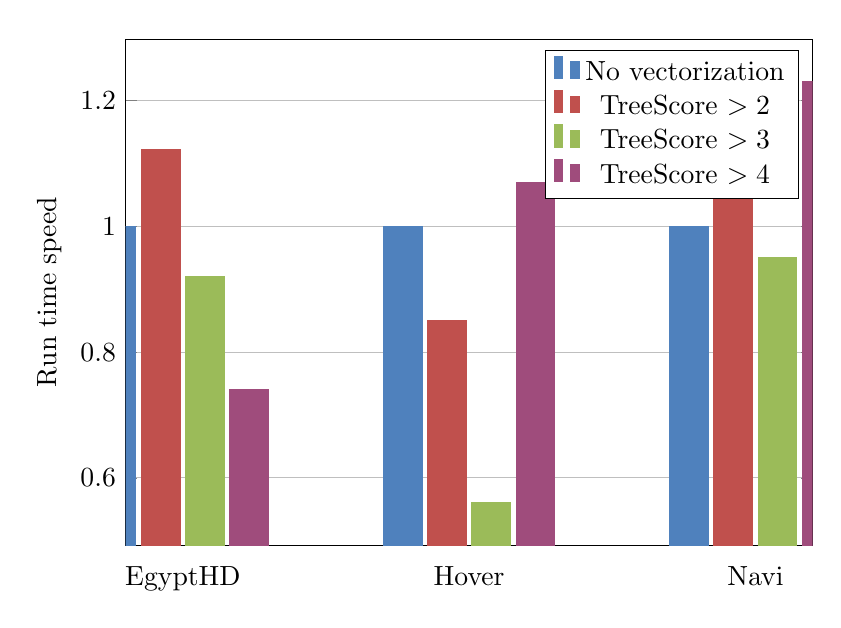
\begin{tikzpicture}
    \begin{axis}[
        width  = 0.85*\textwidth,
        height = 8cm,
        major x tick style = transparent,
        ybar,
        bar width=14pt,
        ymajorgrids = true,
        ylabel = {Run time speed},
        symbolic x coords={EgyptHD,Hover,Navi},
        xtick = data,
        scaled y ticks = false,
    ]
        \addplot[style={bblue,fill=bblue,mark=none}]
            coordinates {(EgyptHD, 1.0) (Hover,1.0) (Navi,1.0)};

        \addplot[style={rred,fill=rred,mark=none}]
             coordinates {(EgyptHD,1.123) (Hover,0.85) (Navi,1.09)};

        \addplot[style={ggreen,fill=ggreen,mark=none}]
             coordinates {(EgyptHD,0.92) (Hover,0.56) (Navi,0.95)};

        \addplot[style={ppurple,fill=ppurple,mark=none}]
             coordinates {(EgyptHD,0.74) (Hover,1.07) (Navi,1.23)};

        \legend{No vectorization,TreeScore $>2$,TreeScore $>3$,TreeScore $>4$}
    \end{axis}
\end{tikzpicture}
\end{document}